% Options for packages loaded elsewhere
\PassOptionsToPackage{unicode}{hyperref}
\PassOptionsToPackage{hyphens}{url}
\PassOptionsToPackage{dvipsnames,svgnames,x11names}{xcolor}
%
\documentclass[
  10pt,
]{article}
\usepackage{amsmath,amssymb}
\usepackage{iftex}
\ifPDFTeX
  \usepackage[T1]{fontenc}
  \usepackage[utf8]{inputenc}
  \usepackage{textcomp} % provide euro and other symbols
\else % if luatex or xetex
  \usepackage{unicode-math} % this also loads fontspec
  \defaultfontfeatures{Scale=MatchLowercase}
  \defaultfontfeatures[\rmfamily]{Ligatures=TeX,Scale=1}
\fi
\usepackage{lmodern}
\ifPDFTeX\else
  % xetex/luatex font selection
\fi
% Use upquote if available, for straight quotes in verbatim environments
\IfFileExists{upquote.sty}{\usepackage{upquote}}{}
\IfFileExists{microtype.sty}{% use microtype if available
  \usepackage[]{microtype}
  \UseMicrotypeSet[protrusion]{basicmath} % disable protrusion for tt fonts
}{}
\makeatletter
\@ifundefined{KOMAClassName}{% if non-KOMA class
  \IfFileExists{parskip.sty}{%
    \usepackage{parskip}
  }{% else
    \setlength{\parindent}{0pt}
    \setlength{\parskip}{6pt plus 2pt minus 1pt}}
}{% if KOMA class
  \KOMAoptions{parskip=half}}
\makeatother
\usepackage{xcolor}
\usepackage[margin=1in]{geometry}
\usepackage{graphicx}
\makeatletter
\def\maxwidth{\ifdim\Gin@nat@width>\linewidth\linewidth\else\Gin@nat@width\fi}
\def\maxheight{\ifdim\Gin@nat@height>\textheight\textheight\else\Gin@nat@height\fi}
\makeatother
% Scale images if necessary, so that they will not overflow the page
% margins by default, and it is still possible to overwrite the defaults
% using explicit options in \includegraphics[width, height, ...]{}
\setkeys{Gin}{width=\maxwidth,height=\maxheight,keepaspectratio}
% Set default figure placement to htbp
\makeatletter
\def\fps@figure{htbp}
\makeatother
\setlength{\emergencystretch}{3em} % prevent overfull lines
\providecommand{\tightlist}{%
  \setlength{\itemsep}{0pt}\setlength{\parskip}{0pt}}
\setcounter{secnumdepth}{-\maxdimen} % remove section numbering
\usepackage{graphicx}
\usepackage{mathrsfs}
\usepackage{float}
\floatplacement{figure}{H}
\usepackage{microtype}
\setlength{\emergencystretch}{2em}
\setlength{\parskip}{4pt}
\setlength{\parindent}{0pt}
\AtBeginDocument{\author{Ricardo Maldonado\\Independent Researcher\\
ORCID: 0009-0009-3937-6527\\
\texttt{ricardomaldonadoandrade@gmail.com}}}
\ifLuaTeX
  \usepackage{selnolig}  % disable illegal ligatures
\fi
\usepackage{bookmark}
\IfFileExists{xurl.sty}{\usepackage{xurl}}{} % add URL line breaks if available
\urlstyle{same}
\hypersetup{
  pdftitle={Regular cone evolution and local symplectic flux in an Einstein--scalar shell model},
  pdfauthor={Ricardo Maldonado},
  colorlinks=true,
  linkcolor={Maroon},
  filecolor={Maroon},
  citecolor={Blue},
  urlcolor={Blue},
  pdfcreator={LaTeX via pandoc}}

\title{Regular cone evolution and local symplectic flux in an
Einstein--scalar shell model}
\author{Ricardo Maldonado}
\date{13 October 2026 --- technical draft for author review}

\begin{document}
\maketitle
\begin{abstract}
A singular radial master variable can obscure regular evolution across a
characteristic cone. For the nonconstant regular branch of a fixed
five-dimensional Einstein--scalar shell model, we derive an equivalent
ambient master equation with smooth coefficients and Minkowski principal
symbol. An explicit local differential reconstruction gives metric and
scalar perturbations smooth at the cone and its vertex. Direct field
equation identities prove sufficiency without division by a tangential
harmonic eigenvalue. Standard normally hyperbolic Cauchy theory then
constructs actual coupled perturbations from smooth compact data. Before
their support reaches the shell, either reflection parity satisfies the
homogeneous junction conditions with zero shell displacement. An exact
angular-harmonic Cauchy-jet construction gives two non-gauge solutions
with nonzero local Einstein--scalar null symplectic flux. This closes a
local solution-existence gap in the preceding conditional flux result.
The physical Cauchy symplectic form is also nondegenerate on the image
of smooth master data supported in a sufficiently small spatial ball.
Evolution after shell contact, global phase-space completeness,
nonlinear stability and cosmological interpretation remain open.
\end{abstract}

\textbf{Status.} Reproducible technical continuation, not an APS
submission or external peer review. The novelty comparison is bounded;
no claim of worldwide priority or evidence for a higher-dimensional Big
Bang is made.

\section{1. Question and fixed
background}\label{question-and-fixed-background}

The preceding checkpoint {[}1{]} derived the actual
gravitational--scalar symplectic current and its cone limit, conditional
on actual solutions having differentiable characteristic expansions. Its
explicit nonzero-flux example was a separate flat test-scalar problem.
Here we construct a family of solutions of the registered coupled
equations that realizes nonzero flux. The result is local in ambient
time and uses finite propagation to meet the shell conditions before
contact. It does not solve the subsequent initial-boundary-value
problem.

Use signature \((-++++)\), \(8\pi G_5=1\), and the doubled-interior
action \[
 S=\sum_{i=\pm}\left\{\int_{M_i}\!\epsilon_g
 [R/2-(\nabla\phi)^2/2-U(\phi)]+\int_\Sigma\!\epsilon_hK_i\right\}
 -\int_\Sigma\!\epsilon_h\sigma(\phi).                         \tag{1}
\] Both outward shell normals point toward increasing interior radius.
The registered functions and detuning interval are \[
 \begin{gathered}
 \eta=\phi-1,\quad W=\tfrac13+\eta^2+\tfrac13\eta^3,\quad
 U=\tfrac12W_{,\phi}^2-\tfrac23W^2,\\
 \sigma=2W+\delta(1+c+c\eta),\quad
 c=\frac2{1.0357712571566784}-\frac43,\quad0<\delta\le0.002.
 \end{gathered}                                               \tag{2}
\] The decimal is exact. Fix one background on the already certified
regular branch {[}2{]}; this note does not recertify that branch or take
a uniform \(\delta\to0\) limit. Its warped form and equations are \[
 g=dy^2+\rho(y)^2\gamma,\quad\operatorname{Ric}\gamma=3\gamma,
 \quad a=\rho'/\rho,\quad p=\phi',
\] \[
 p'=U_{,\phi}-4ap,\quad a'=-\rho^{-2}-p^2/3,\quad
 a^2=\rho^{-2}+p^2/12-U/6,
 \qquad a_b=\sigma_b/6,\quad p_b=-\sigma_{,\phi,b}/2.             \tag{3}
\] The regular endpoint has \(\rho=y+O(y^3)\), \(p=\kappa y+O(y^3)\),
\(\kappa\ne0\), with analytic coefficients in \(y^2\). On this fixed
branch \(p<0\) for \(0<y\le T_b\). Analyticity is used to extend the
background across the cone. The perturbations themselves need only be
smooth.

Introduce the exact conformal radius by \[
 \frac{dr}{r}=\frac{dy}{\rho},\quad r/y\longrightarrow1,\quad
 s=r^2=X\cdot X,\quad g_{AB}=\Omega(s)^2\eta_{AB},\quad
 \rho=r\Omega(s),\quad\phi=\Phi(s),\quad f=\Phi_s.               \tag{4}
\] Here \(X=(T,\mathbf X)\), \(R=|\mathbf X|\), \(s=R^2-T^2\), and
\(\Omega(0)=1\), \(f(0)=\kappa/2\ne0\). Analytic continuation gives a
neighborhood \(-\epsilon<s<s_+\) with \(\Omega>0\), \(f\ne0\); the
background equations continue there. This is a local Lorentzian
extension, not a singular creation surface. Define \[
 E=X^A\partial_A,\qquad
 L=\frac{\Omega_s}{\Omega}+2\frac{f_s}{f},\qquad
 \mathcal L=\Box_\eta-2L(s)E-
 \left[8L(s)+\frac83sf(s)^2\right].                            \tag{5}
\]

\section{2. Exact regular master and
reconstruction}\label{exact-regular-master-and-reconstruction}

In the longitudinal scalar slice write \(h_{yy}=-4\Psi\),
\(h_{y\mu}=0\), \(h_{\mu\nu}=2\rho^2\Psi\gamma_{\mu\nu}\), and
\(\delta\phi=\chi\). The inherited unreduced master is \[
 P=\rho^2\Psi,\quad\chi=-\frac{3P_y}{\rho^2p},\qquad
 M[P]=P_{yy}-(2a+2p'/p)P_y+
 \rho^{-2}(\Box_\gamma+4)P-\frac23p^2P.                         \tag{6}
\] The expression appears singular because \(p\) vanishes at the
endpoint. Set \[
                         P=r^4F(X).                           \tag{7}
\] Using \(\partial_y=\Omega^{-1}\partial_r\), \(p=2rf/\Omega\) and
\(\Box_\eta=\partial_r^2+4\partial_r/r+\Box_\gamma/r^2\) on \(s>0\)
gives the exact identity \[
                   M[r^4F]=\Omega^{-2}r^4\mathcal LF.            \tag{8}
\] The reconstructed fields take the manifestly regular ambient form \[
 \boxed{h_{AB}=2sF\eta_{AB}-6F X_AX_B,\qquad
 \chi=-\frac{3}{2\Omega^2f}(E+4)F.}                            \tag{9}
\] Indices on \(X\) in this expression are lowered with \(\eta\). For
example, \(dy^2=\Omega^2(X_A dX^A)^2/s\); cancellation with
\(\Psi=sF/\Omega^2\) removes its apparent pole. Equation (9) is smooth
even at \(X=0\).

\textbf{Proposition 1 (sufficient coupled solution family).} Every
smooth solution \(F\) of \(\mathcal LF=0\) in the extended background
reconstructs through (9) a solution of all linearized bulk Einstein and
scalar equations. No completeness assertion is made about arbitrary
gravitational perturbations or exceptional scalar harmonic sectors.

\textbf{Proof.} Define the trace-reversed Einstein and scalar residuals
by \[
 \mathscr E_{AB}=R_{AB}-\phi_{,A}\phi_{,B}-\tfrac23Ug_{AB},
 \qquad\mathscr S=\Box_g\phi-U_{,\phi}.
\] Direct metric variation, followed only by (3) and the reconstruction,
gives \[
 \delta\mathscr E_{yy}=2M[P]/\rho^2,\quad
 \delta\mathscr E_{y\mu}=0,\quad
 \delta\mathscr E_{\mu\nu}=-\gamma_{\mu\nu}M[P],
\] \[
 \delta\mathscr S=-\frac3{\rho^2p}(\partial_y+2a)M[P].           \tag{10}
\] Equivalently, in ambient coordinates, \[
 \boxed{\delta\mathscr E_{AB}=
 \Omega^{-2}(3X_AX_B-s\eta_{AB})\mathcal LF,\qquad
 \delta\mathscr S=-\frac3{2\Omega^4 f}(E+6)\mathcal LF.}          \tag{11}
\] These are differential-operator identities. Their coefficients extend
analytically in \(s\), so identities established for \(s>0\) continue
across \(s=0\) and hold for arbitrary smooth test \(F\). All residuals
vanish when \(\mathcal LF=0\). No division by \(\Box_\gamma+4\) or by a
separated eigenvalue occurs. The accompanying direct-index checker
verifies all 15 independent Ricci components and the scalar variation; a
separate ADM calculation checks the constraints and scalar equation.
\(\square\)

\section{3. Cauchy existence, finite energy and the
shell}\label{cauchy-existence-finite-energy-and-the-shell}

The principal symbol of \(\mathcal L\) is precisely that of
five-dimensional Minkowski space. Its lower-order coefficients are
smooth where \(f\ne0\). Standard normally hyperbolic Cauchy theory
{[}3{]} therefore supplies a unique smooth local solution for any smooth
compact initial data \((F,F_T)\) on a spacelike slice \(T=t_0\), with
propagation speed at most one. One may extend the coefficients smoothly
outside a compact causal neighborhood, solve the auxiliary Cauchy
problem, and restrict back. Domain of dependence makes the restricted
solution independent of that extension.

For an explicit energy estimate, the positive weight
\(A=(\Omega f^2)^{-1}\) satisfies \(A_s/A=-L\). With \(\psi=\sqrt A F\),
equation (5) is equivalent to \[
 (\Box_\eta-V_c)\psi=0,\qquad
 V_c=3L-2sL_s+sL^2+\tfrac83sf^2.                              \tag{12}
\] On a compact time slab containing the causal support, let
\(K=\sup|1-V_c|\). The auxiliary energy \[
 \mathcal E(T)=\frac12\int_{\mathbb R^4}
 (|\psi_T|^2+|\nabla\psi|^2+|\psi|^2)d^4X
\] satisfies \(|\mathcal E'|\le K\mathcal E\), hence
\(\mathcal E(T)\le\mathcal E(t_0)e^{K|T-t_0|}\). Smooth coefficients and
commuted estimates preserve smoothness. This is a control norm for the
master equation. It is not identified with the gravitational symplectic
norm, a conserved physical energy, or a proof of absence of
gravitational ghosts. Smooth compact reconstructed fields have finite
local norms; derivative reconstruction changes the required Sobolev
order.

\textbf{Proposition 2 (short-time doubled-shell solutions).} Suppose the
causal support of compact initial data stays within a region of the
analytically extended fixed background and remains a positive distance
from the shell for \(|T-t_0|<\Delta\). Then (9), with either even or odd
copying to the second interior and zero shell displacement, solves the
full homogeneous linearized bulk and junction equations on that slab.

\textbf{Proof and usable criterion.} The shell is the timelike
hyperboloid \(R_b(T)=\sqrt{r_b^2+T^2}\), with \(r_b=r(T_b)>0\). Data
supported in \(R\le R_0\) propagate inside \(R\le R_0+|T-t_0|\). Thus
\(R_0+\Delta<r_b\) ensures an open zero-field neighborhood of the shell.
All local derivatives of the reconstructed fields vanish there. With
zero displacement, every linearized matching residual vanishes,
including the scalar junction and the moving-shell terms. The bound
\((|t_0|+\Delta)^2<\epsilon\) keeps the timelike part in the available
background extension; alternatively choose the whole support in an even
smaller cone neighborhood. The positive-\(s\) support must also remain
in the actual background interval, for example by
\((R_0+\Delta)^2<s_+\). The field may be set to zero beyond that
neighborhood where its causal support is absent. The construction works
for each parity. \(\square\)

One explicit choice also includes the cone vertex. If the actual
analytic coefficient neighborhood contains \(|s|<\sigma\), choose
\(t_0>0\) so that \(13t_0^2<\sigma\) and \(4t_0<r_b\), and initial
support in \(t_0/2<R<3t_0/2\). On \(-t_0<T<3t_0\), its causal support
obeys \(R\le7t_0/2\) and hence \(|s|<13t_0^2\). It remains strictly
inside the shell throughout this slab, which contains both the vertex
and the finite cone cut used below. Subsequent support reaching \(R=0\)
causes no problem for smooth Cartesian Cauchy evolution.

\begin{figure}
\centering
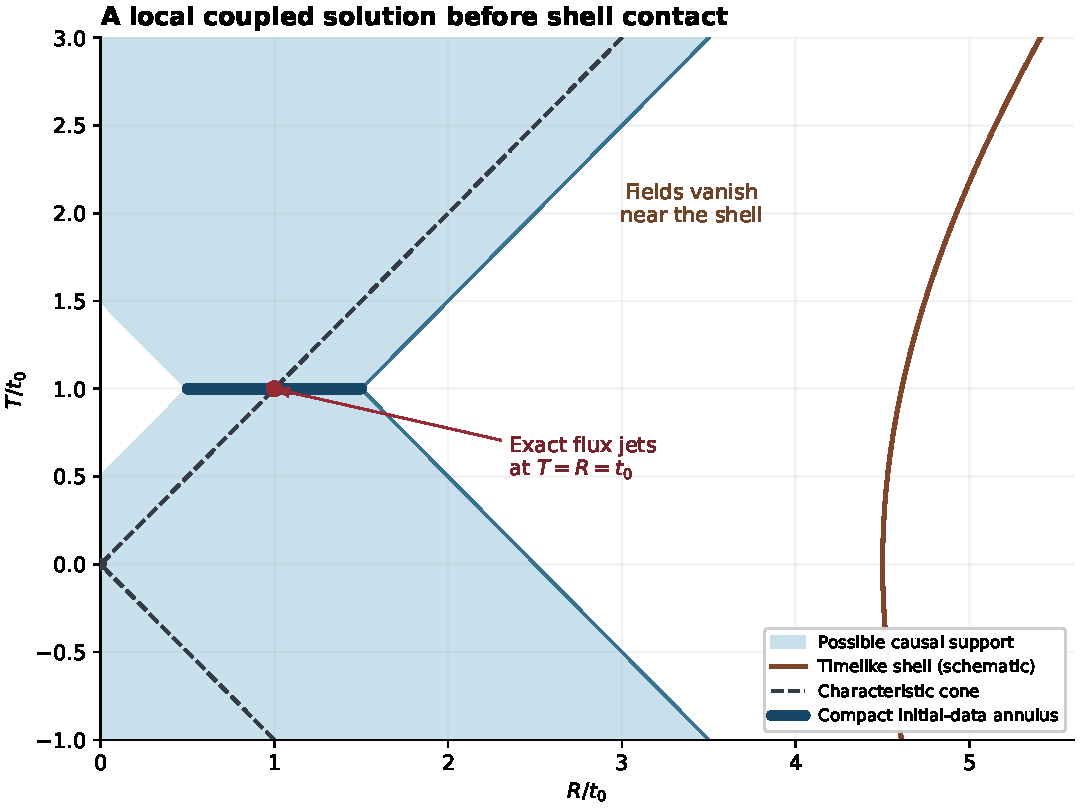
\includegraphics[width=0.85\textwidth,height=\textheight]{../figures/support-geometry.pdf}
\caption{Finite-propagation geometry, in units of the chosen local time
scale. The illustrative shell ratio is \(r_b/t_0=4.5\); this is a
geometric schematic, not a numerical background or perturbation
solution. The shading bounds possible support, not wave amplitude.}
\end{figure}

This result deliberately ends before shell contact. It provides no
reflection law, all-time Wentzell evolution, boundary compatibility
hierarchy after contact, or global Hilbert-space identification. Prior
scalar Wentzell results {[}4{]} and current vacuum Einstein boundary
theorems {[}5,6{]} do not by themselves supply the required coupled
Israel-shell theorem.

\section{4. Actual non-gauge solutions with nonzero cone
flux}\label{actual-non-gauge-solutions-with-nonzero-cone-flux}

Let \(u=R-T\), \(v=R+T\), so \(s=uv\). Work on a finite future-cone
segment \(u=0\), \(v>0\), away from its vertex. Smoothness of \(F\) in
(9) supplies the uniform differentiated expansions required in {[}1{]}.
Its limiting scalar is \[
 \chi_0(v,\vartheta)=-C(4+v\partial_v)F_0(v,\vartheta),
 \qquad C=\frac3{2f(0)}=\frac3\kappa.                         \tag{13}
\] For the convention of increasing radial normal, the per-copy current
density tends to \[
 \frac{v^3}{8}(\chi_{01}\partial_v\chi_{02}
              -\chi_{02}\partial_v\chi_{01})\,dv\,d\Omega_3.
                                                                    \tag{14}
\] Taking both solutions with the same reflection parity, either even or
odd, gives twice (14); a mixed-parity pair cancels between copies. This
is the actual Einstein--scalar symplectic current restricted to this
solution family, not the auxiliary current of (12). It is antisymmetric
in the two solutions and is not a positive energy flux.

We now construct its nonzero value directly from freely specified Cauchy
data, without assuming a characteristic boundary-value theorem. Fix
small \(t_0>0\), and let \(H_l\) be a real unit-normalized spherical
harmonic on \(S^3\), \(\Delta_{S^3}H_l=-\lambda H_l\),
\(\lambda=l(l+2)\), \(l\ge2\). Take a smooth radial cutoff \(\zeta(R)\)
supported in an annulus about \(R=t_0\) and equal to one near that
sphere. Specify at \(T=t_0\) \[
 F_1=a\zeta H_l,\quad F_{1T}=0,\qquad
 F_2=0,\quad F_{2T}=b\zeta H_l,\qquad ab>0.                    \tag{15}
\] The annulus makes these smooth compact Cartesian data. Rotational
invariance preserves \(l\); \(l\ge2\) also avoids the constant and
Hessian-degenerate harmonic subspaces relevant to the earlier scalar
reduction. Choose its support and the slab to satisfy Proposition 2.

At \(T=R=t_0\) (\(v_0=2t_0\)), put \(L_0=L(0)\). Equation (5) fixes the
second time derivatives: \[
 F_{1TT}=-(\lambda/t_0^2+8L_0)aH_l,
 \qquad F_{2TT}=-2L_0t_0bH_l.
\] Since \(\partial_v=(\partial_T+\partial_R)/2\) and \(\partial_vs=0\)
on the cone, the reconstructed jets are exactly \[
 \begin{aligned}
 \chi_1&=-4CaH_l,&
 \chi_{1v}&=Ca[\lambda/(2t_0)+4t_0L_0]H_l,\\
 \chi_2&=-Ct_0bH_l,&
 \chi_{2v}&=-Cb[5/2-t_0^2L_0]H_l.
 \end{aligned}                                                \tag{16}
\] Consequently, \[
 \boxed{\chi_1\chi_{2v}-\chi_2\chi_{1v}
       =C^2ab(10+\lambda/2)H_l^2.}                            \tag{17}
\] The background-dependent terms cancel. For \(l=2\), the coefficient
is \(14C^2ab\). After angular integration the doubled current density at
\(v_0\) is \(28t_0^3C^2ab>0\). Continuity makes the integrated flux
strictly nonzero on a sufficiently short \(v\) interval around \(v_0\).
Its sign can be reversed by exchanging the two solutions, as a
symplectic bilinear must.

Nonzero current alone is not a gauge-invariance test at a null boundary.
For a separate physical witness, use the background scalar
\(K_g=(\nabla\phi)^2=4sf^2/\Omega^2\) and its relational perturbation \[
 Z=\delta K_g-\frac{(K_g)_s}{f}\chi.                          \tag{18}
\] It is invariant under smooth infinitesimal diffeomorphisms: the two
background Lie derivatives cancel. On the cone it equals
\(Z=4f(0)(v\chi_v-\chi)\). For (16), \[
 \begin{aligned}
 Z_1&=4f(0)Ca[\lambda+4+8t_0^2L_0]H_l,\\
 Z_2&=4f(0)Ct_0b[-4+2t_0^2L_0]H_l.
 \end{aligned}                                                \tag{19}
\] Choosing \(l=2\) and \(|t_0^2L_0|<1\) makes both nonzero functions.
Thus each solution is non-pure-gauge under smooth diffeomorphisms. This
does not classify finite-cut gauge charges or prove that the current
descends to a complete global quotient.

\section{5. Prior work, verification and remaining
questions}\label{prior-work-verification-and-remaining-questions}

Regular normally hyperbolic Cauchy evolution is established mathematics
{[}3{]}. Gauge-invariant scalar master variables in gravitating walls
and brane stabilization have substantial prior literature {[}7,8{]}.
Their variables and zero-set hypotheses must be compared before using
them at the cone. In particular, a variable containing \(1/\phi'\) is
not made regular merely by calling it gauge invariant. The present
calculation supplies an explicit transformation, smooth reconstruction
and full residual factorization for the fixed branch (2).

Earlier private HDBLAST notes M465R1 and M471 already discussed regular
ambient evolution and cone transparency for a branch near \(\phi=-1\).
Their conceptual observation is acknowledged. Their negative-branch
numerical focusing bounds and stationary transfer conclusion do not
transfer to the present branch near \(\phi=+1\). The added result here
is the specific regular master, reconstruction, exact non-gauge flux
pair and finite-time shell argument for the registered current model.
The accompanying literature register records the bounded searches,
selected primary passages, and exclusions; it does not establish
external originality.

The capsule includes separate direct-index and ADM derivations, exact
symbolic checks, deliberately wrong formulas, normal and optimized
Python reproduction, and integrity verification. These checks support
the stated algebra. The analytic Cauchy theorem, support argument and
proof hypotheses are necessary parts of the result; check counts are not
counts of independent physical discoveries. No numerical evolution or
observational fit is presented.

The next decisive task is to evolve these smooth data through first
shell contact with the correct coupled junction conditions and energy
estimate. A subsequent task is to identify the allowed gauge quotient
and compare its physical phase space with the earlier radial spectral
closure. Neither the existence result here nor the positive radial
theorem alone settles that comparison. Nonlinear evolution, reheating,
cosmological observables and discrimination from four-dimensional rivals
remain open. The proposed higher-dimensional origin of the Big Bang
remains unestablished.

\section{Appendix A. Exact boundary laws and a local Cauchy
form}\label{appendix-a.-exact-boundary-laws-and-a-local-cauchy-form}

The supplemental boundary audit supplies two further precise statements.
At the fixed shell define \(B_b=p'_b/p_b+\sigma''_b/2>0\). Transforming
the inherited master junctions by \(P=r^4F\) gives \[
 nF-B_b^{-1}\Box_{h_b}F+
 \left(\frac4{\rho_b}-\frac4{\rho_b^2B_b}\right)F=0
 \quad\hbox{(even)},
\] \[
 nF+\left(\frac4{\rho_b}+\frac{p_b^2}{3a_b}\right)F=0
 \quad\hbox{(odd)},                                      \tag{20}
\] where \(n=\partial_y\) is the outward physical normal. The first
equation has a tangential wave operator (a Wentzell condition); the
second is Robin. Their exact conversion is useful for the next evolution
problem. It does not prove that problem well posed after contact, and
the positive boundary kinetic coefficient of an auxiliary master action
is not identified with the physical Einstein--scalar boundary kinetic
form.

For a separate bounded phase-space result, take smooth real compact
master data \((q,p)=(F,F_T)|_{T=0}\) in a sufficiently small ball. Here
\(p\) denotes initial velocity only, not the background radial
derivative in (3). Put \(D_r=r\partial_r\) and
\(m_r=9r^3/(4\Omega f^2)\). The actual per-copy Einstein--scalar
current, with future Cauchy orientation, pulls back to \[
 \sigma((q_1,p_1),(q_2,p_2))=K(q_1,p_2)-K(q_2,p_1),
\] \[
 K(q,p)=\int dr\,d\Omega_3
 \left[m_r(D_r+4)q(D_r+5)p+\frac{6r^7}{\Omega}qp\right].       \tag{21}
\] Indeed \(\chi=-3(D_r+4)q/(2\Omega^2f)\) and
\(\chi_T=-3(D_r+5)p/(2\Omega^2f)\) on this slice; the extra unit follows
from \([\partial_T,E]=\partial_T\). Transforming the physical time
current gives the measure \(\Omega^3r^3\). Compact-support integration
by parts, using \(r\partial_r\log m_r=3-2sL\), yields \[
 K(q,q)=\int dr\,d\Omega_3
 \left[m_r\{(D_rq)^2+(2+9sL)q^2\}
       +\frac{6r^7}{\Omega}q^2\right].                       \tag{22}
\] Choose the ball so that \(2+9sL\ge1\). Then \(K(q,q)>0\) for every
nonzero \(q\). A pair in the kernel of \(\sigma\) against all compact
test pairs must have \(q=0\) by testing against \((0,q)\), and then
\(p=0\) by testing against \((p,0)\). Thus this physical pullback is
nondegenerate on the stated smooth compact master-data image. \(K\)
itself need not be symmetric. The result does not identify a completed
Hilbert space, a global gravitational Hamiltonian, or the full gauge
quotient. The shell contribution vanishes here because the data have
support away from the shell.

\section{Declarations and
availability}\label{declarations-and-availability}

Ricardo Maldonado, Independent Researcher; ORCID 0009-0009-3937-6527. No
funding. No known competing interests. The earlier author declaration
states that the manuscript is not under consideration elsewhere. No new
APS submission accompanies this continuation, and the prior DX13808
rejection is not reversed by these calculations.

Substantial OpenAI Codex assistance was used for mathematical
derivation, symbolic programming, literature organization, internal
review and drafting. Separate agent processes supplied internal checks;
they are not external human peer review. The author retains
responsibility for review and any submission. Source, code, exact
receipts and this draft are supplied in the associated GitHub research
capsule; the preceding spectral edition is archived at DOI
10.5281/zenodo.23335485 within concept DOI 10.5281/zenodo.17088132.

\section{References}\label{references}

\begin{enumerate}
\def\labelenumi{\arabic{enumi}.}
\tightlist
\item
  R. Maldonado, \emph{Covariant flux and physical-domain limits of
  regular de Sitter shells}, HDBLAST technical checkpoint (13 October
  2026),
  \href{https://github.com/maldonado-research/HDblast/tree/a3757e563dbfd5c9a3fded4d50674bacaf6cafb5/research/HDBLAST_CONE_PHASE_SPACE_20261013}{immutable
  source}.
\item
  R. Maldonado, \emph{From scalar-boundary Jacobi response to spectral
  positivity of regular de Sitter shells}, technical note in the HDBLAST
  regular-shell spectral checkpoint (13 October 2026),
  \href{https://doi.org/10.5281/zenodo.23335485}{doi:10.5281/zenodo.23335485}.
\item
  C. Bär and R. Tagne Wafo, \emph{Initial value problems for wave
  equations on manifolds}, Math. Phys. Anal. Geom. \textbf{18}, 7
  (2015), \href{https://arxiv.org/abs/1408.4995v2}{arXiv:1408.4995v2},
  especially Theorem 13 and Corollary 14. The cited theorem applies
  after smoothness and normal hyperbolicity have been established.
\item
  J. Zahn, \emph{Generalized Wentzell boundary conditions and quantum
  field theory}, Ann. Henri Poincaré \textbf{19}, 163--187 (2018),
  \href{https://arxiv.org/abs/1512.05512v3}{arXiv:1512.05512v3}. Scalar
  dynamic-boundary comparator, not a coupled Israel-shell theorem.
\item
  Z. An and M. T. Anderson, \emph{Well-posed geometric boundary data in
  General Relativity, II: Twisted Dirichlet boundary data}, Class.
  Quantum Grav. \textbf{43}, 115020 (2026),
  \href{https://arxiv.org/abs/2507.15567v3}{arXiv:2507.15567v3}. Its
  vacuum theorem includes five dimensions, but its boundary conditions
  and matter content differ from this model.
\item
  C. Stevens and J. A. Valiente Kroon, \emph{Wellposedness of the
  initial boundary value problem for the conformal field equations},
  \href{https://arxiv.org/abs/2604.24931v1}{arXiv:2604.24931v1}. Used
  for comparison of four-dimensional vacuum-boundary scope, not as a
  proof of the present shell evolution. Its general two-coefficient
  estimate (32) is not used.
\item
  M. Giovannini, \emph{Gauge-invariant fluctuations of scalar branes},
  Phys. Rev.~D \textbf{64}, 064023 (2001),
  \href{https://arxiv.org/abs/hep-th/0106041v1}{arXiv:hep-th/0106041v1}.
\item
  D. Konikowska, M. Olechowski and M. G. Schmidt, \emph{Radion
  stabilization with(out) Gauss--Bonnet interactions and inflation},
  \href{https://arxiv.org/abs/hep-th/0603014v2}{arXiv:hep-th/0603014v2}.
  The scalar-zero variable and finite-interval stability hypotheses
  differ from the present cone; the exact scope and printed-variable
  caveat are recorded in the accompanying primary-source register.
\end{enumerate}

\end{document}
